% CVPR 2026 Paper Template; see https://github.com/cvpr-org/author-kit

\documentclass[10pt,twocolumn,letterpaper]{article}

%%%%%%%%% PAPER TYPE  - PLEASE UPDATE FOR FINAL VERSION
% \usepackage{cvpr}              % To produce the CAMERA-READY version
\usepackage[review]{cvpr}      % To produce the REVIEW version
% \usepackage[pagenumbers]{cvpr} % To force page numbers, e.g. for an arXiv version

% Import additional packages in the preamble file, before hyperref
\input{preamble}

% It is strongly recommended to use hyperref, especially for the review version.
% hyperref with option pagebackref eases the reviewers' job.
% Please disable hyperref *only* if you encounter grave issues, 
% e.g. with the file validation for the camera-ready version.
%
% If you comment hyperref and then uncomment it, you should delete *.aux before re-running LaTeX.
% (Or just hit 'q' on the first LaTeX run, let it finish, and you should be clear).
\definecolor{cvprblue}{rgb}{0.21,0.49,0.74}
\usepackage[pagebackref,breaklinks,colorlinks,allcolors=cvprblue]{hyperref}
\input{math_commands.tex}

\usepackage{hyperref}
\usepackage{url}
\usepackage{float}
\usepackage{epsfig}
\usepackage{graphicx}
\usepackage{amsmath}
\usepackage{amssymb}
\usepackage{subcaption}
\usepackage{placeins}
\usepackage{makecell}
\usepackage{xcolo r}
\usepackage{booktabs}
\usepackage{dsfont}
\usepackage{multirow}

%%%%%%%%% PAPER ID  - PLEASE UPDATE
\def\paperID{*****} % *** Enter the Paper ID here
\def\confName{CVPR}
\def\confYear{2026}


\title{\textbf{ReefFormer:} Global disentangled dense segmentation of coral reef imagery %/Explainable/Concept-decomposed
}


\author{
First Author\\
Institution1\\
Institution1 address\\
{\tt\small firstauthor@i1.org}
% For a paper whose authors are all at the same institution,
% omit the following lines up until the closing ``}''.
% Additional authors and addresses can be added with ``\and'',
% just like the second author.
% To save space, use either the email address or home page, not both
\and
Second Author\\
Institution2\\
First line of institution2 address\\
{\tt\small secondauthor@i2.org}
}

\begin{document}
\maketitle
\begin{abstract}
Coral reefs are existentially threatened by anthropogenic climate change and local stressors: their collapse is devastating for biodiversity and threatens the livelihoods of coastal communities that depend on reefs. However, there are substantial gaps in the understanding of the dynamics underlying reef degradation and recovery: to fill these gaps and to inform effective conservation and restoration measures, coral reef monitoring needs to be scaled up to the highest resolution possible. As an unprecedented volume of imagery is collected for coral reef monitoring, machine learning promises to overcome the data analysis bottleneck of large-scale monitoring efforts.
However, current machine learning tools and datasets are highly fragmented across ecoregions, image types (e.g. photo quadrats, orthomosaics, or casual images), and labelsets. In this paper we reconcile highly heterogeneous public coral reef imagery from 7 datasets into a joint label space disentangled into concepts that explicitly model the multi-hierarchy of the benthos, and establish the first rigorous benchmark that spans ecoregions, taxonomy, coral health and morphology across both sparse and dense annotations. On this reconciled dataset, we train \emph{ReefFormer}, a unified foundation model for dense segmentation of reef imagery that generalizes across to reefs worldwide across all aspects of the disentangled prediction space. The experiments across the benchmark reveal a trade-off between data quality and quantity, highlighting the need for high-quality datasets. ReefFormer serves as a foundation model in computer vision for reefs: it can be used and fine-tuned flexibly in a wide range of coral reef monitoring use cases, and accelerate further research in the coral reefs and other ecological domains.
\end{abstract}


\section{Introduction}

%- coral reefs are existentially threatened - (add principal well-established references)\\
%- very briefly explain that heat stress leads to mass bleaching, which leads to mass mortality if prolonged.\\
%- current GHG emission trajectories will likely lead to loss of \% of coral
%- coral is at the base of the coral reef ecosystem: mass mortality leads to biodiversity collapse and catastrophic impacts for coastal communities\\
%- precise dynamics of reef degradation and recovery vary regionally and are not well understood\\
%- coral monitoring needs to be scaled up, - with many references - clearly motivate this, we need it to inform effective conservation or restoration action!\\
%- The computer vision in coral reefs community 

Coral reefs are severely threatened by anthropogenic climate change and local stressors \citep{hughes2017anthropocene,cooley2022oceans}. Marine heatwaves cause mass bleaching of corals, which can lead to widespread mortality when thermal stress is severe or prolonged \citep{hughes2017global}. Under current greenhouse-gas emission trajectories, it is estimated that more than 99\% of reef-building coral may be lost by 2100 \citep{ipcc2023ar6syr}. Because reef-building corals are the foundation of coral reef ecosystems, their loss is not only catastrophic for biodiversity, but also impacts ecosystem services depended on by many coastal communities \citep{graham2013importance,woodhead2019coral}.
\begin{figure*}[t!]
    \centering
    \includegraphics[width=0.99\linewidth]{overview.png}
    \caption{    We reconcile highly heterogeneous into a unified disentangled label space covering taxonomy, coral morphology, health, and auxiliary concepts. On this meta-dataset, we train ReefFormer for multi-hierarchical dense benthic segmentation.}
    \label{fig:overview}
\end{figure*}

Patterns of degradation and recovery vary substantially among regions and remain incompletely understood \citep{graham2015predicting,darling2019social}. Effective conservation and restoration therefore require monitoring at greater spatial, temporal, and taxonomic resolution \citep{obura2019monitoring}. However, computer vision in the coral reef domain is highly fragmented across platforms, tools, and annotation strategies, effectively restricting the scalability of visual survey analysis and limiting transfer across ecoregions, studies, and monitoring programs.

Annotating corals is extremely challenging: reef imagery contains complex assemblages of algae, sponges, tunicates, fish, crustaceans, mollusks, bacterial mats, and many more.
Even correctly distinguishing coral from non-coral requires substantial knowledge and experience in marine biology. Identifying benthic taxa beyond broad classes often requires dedicated domain experts: 
Corals display high morphological plasticity, the same genus, or even the same species can take various morphologies such as
thin plates, massive, and branching growth forms. On the other hand, corals from different genera can look almost identical. While some charismatic genera or even species can be confidently identified on images by experts, many species or even genera require high-resolution close-ups for identification by trained taxonomists. Some species can simply not be visually identified and require DNA sequencing. Furthermore, coral taxonomy is an active field, with substantial re-assignments within the last years \citep{TODO}. Besides taxonomy, coral can be characterized by their morphology, which drives their ecological function (e.g. branching corals act as nurseries for fish, while massive corals build the principal 3D structure of reefs), and their health status (e.g. bleached, diseased, overgrown by algae). 

Annotated datasets are often driven by needs of the specific studies, and constrained to local biogeography: both the images and label sets of datasets are highly heterogeneous. As an example: one monitoring team might care about globally comparable reef metrics (e.g. live hard coral cover), with images covering large amounts of ground to de-bias the estimate, while coral diversity studies address the heavy tail of what is identifiable, usually working with close-up images to clearly see the corallites. Besides the difference in taxonomic resolution across datasets, there is a quality gradient, ranging from expert taxonomist labels to substantial amounts of annotations coming from volunteers, students, or interns. 

Most publicly available benthic imagery is annotated at sparse points, reflecting established point-count protocols and the interfaces provided by systems such as CoralNet and MERMAID \citep{beijbom2015towards,chen2021new}. Dense annotation datasets exist, but many target individual orthomosaics, binary coral masks, or geographically restricted imagery \citep{yuval2021repeatable,pavoni2022taglab,sauder2024scalable,zheng2024coralscop}. Coralscapes provides a broader dense scene-segmentation benchmark, but remains concentrated in the Red Sea \citep{sauder2025coralscapes}. Dense expert annotations are therefore substantially less abundant and diverse than sparse point labels.


Moreover, the majority of annotated coral reef imagery remains undisclosed: collection and curation are expensive, and access may be constrained by permits, attribution requirements, sensitive locations, institutional ownership, or community governance \citep{obura2019monitoring}.
Conservationists without resources to train their own machine learning systems thus often use platforms that operate under data confidentiality. These platform often provide machine learning models trained on user data, which are a black-box: the users have no control of the models, label classes, or datasets used to train them. Researchers can not independently reproduce or verify results of these models and the reef studies produced with closed models. 
Open models trained on open data are an opportunity to increase the data sovereignty of conservationists and the trustworthiness of the entire chain of automated image analysis in reefs, from individual images to aggregate studies.

In this paper, we reconcile 7 openly available coral reef imagery datasets into a meta-dataset spanning TODO k images and TODO M annotations from TODO %(TODO if you count species) 
taxa. 
We use this meta-dataset to establish a large-scale and rigorous benchmark which spans diverse imagery from biogeographies across the globe, as well as sparse and dense labels. To cover a flexible range of potential downstream use-cases, we disentangle the unified label space into an interpretable set of concepts that cover taxonomy, morphology, health status, and auxiliary concepts relevant to reef science and monitoring. We train and evaluate \textbf{ReefFormer}, a foundation model for dense segmentation of coral reef imagery, demonstrating generalization of reef imagery at global scale.

To summarize, our main contributions are 
\begin{itemize}
   \item We reconcile 7 openly available coral reef imagery datasets: TODO source classes are mapped into a joint space of disentangled interpretable concepts to yield a meta-dataset covering TODOl images, TODO %(TODO if you count species) 
   taxa, and TODO M annotations. The meta-dataset allows rigorous evaluation of the most relevant criteria for benthic segmentation in reefs.
   %TODO: more importantly than our literal dataset and method, we provide a general methodology for extending this in the future.
    \item We directly train dense segmentation models jointly on sparse and dense labels, 
    \item We explore considerations in future data TODO quality blah balh
\end{itemize}

%TODO: emphasize rigor in evaluation!!!
% TODO: recently, there are many papers doing obfuscated things with AI and corals. Instead, we should draw an analogy to megadetector: models with a clearly defined scope that are simple to use and to explain and cover a broad range of use cases can be very impactful.


\section{Related Work}


\paragraph{Reef and benthic segmentation}


%TODO: be inspired by the related work section of Coralscapes (sauder et al., 2025)
%TODO repeat the argument that a clearly defined scope 
Existing methods largely address individual monitoring settings rather than transferable reef understanding. CoralNet and related systems classify patches around sampled points, supporting established cover-estimation protocols but not dense mapping \citep{beijbom2012automated,beijbom2015towards,chen2021coralnet}. Dense methods instead focus on particular domains, including orthomosaics, coral-only masks, or geographically restricted datasets \citep{yuval2021repeatable,pavoni2022taglab,sauder2024deepreefmap,zheng2024coralscop}. Coralscapes broadens dense scene understanding but remains regionally concentrated \citep{sauder2025coralscapes}. Consequently, no existing open model reconciles the geographic, taxonomic, and annotation heterogeneity required for general-purpose reef monitoring.

\paragraph{Dense prediction from sparse labels}

%TODO: all the methods that focus on two-step procedures in the context of coral reefs, where in a first step, labels are densified with some sort of superpixels (recent works by scarlett raine, also coralseg etc.)
%TODO: mention that in coralscape (sauder et al.,), they find that directly training dense segmentation models on sparsified labels outperfroms these methods.

%TODO: this is part of a broader pattern across domains where a lot of annotated data is available as sparse data
%TODO: find papers where training happens directly on sparse labels (outside of the coral/benthic domain)
%TODO Highlight \citep{bokhorst2019learning} explicitly, as they show that a small amount of dense data can complement a large body of sparse data
%TODO 
Sparse point labels are far more abundant than dense reef annotations. Previous coral methods therefore propagate points through superpixels or learned features to create pseudo-masks before training a segmentation network \citep{alonso2017coralsegmentation,alonso2019coralseg,raine2022plas,raine2026hil}. However, segmentation models can also be trained directly by computing their loss only at annotated pixels \citep{bearman2016point,tang2018regularized}. In \citep{sauder2025coralscapes}, this simple strategy was found competitive with coral-specific densification methods in reef settings. %showed in histopathology that limited dense supervision can complement a larger sparse dataset \citep{sauder2025coralscapes,bokhorst2019learning}. ReefFormer builds on these findings by learning directly and jointly from heterogeneous sparse and dense reef annotations.

\section{Dataset Reconciliation}

\begin{table*}[t!]
    \centering
    \resizebox{0.99\textwidth}{!}{%
    \begin{tabular}{lccr|rrr|rrr|rrr}
    \toprule
        \multirow{2}{*}{Dataset}
        & \multirow{2}{*}{\makecell{Annotation\\Type}}
        & \multirow{2}{*}{\makecell{Image\\Type}}
        & \multirow{2}{*}{\makecell{\# Mapped Classes}}
        & \multicolumn{3}{c}{\# Images}
        & \multicolumn{3}{c}{\# Annotations}
        & \multicolumn{3}{c}{\# Annotated Pixels}\\

        & & &
        & Train & Val & Test
        & Train & Val & Test
        & Train & Val & Test
        \\

    \midrule
        Moorea Labeled Corals \citep{beijbom2012automated}
        & Sparse & Photo quadrats & 29
        & 2,002 & 0 & 0
        & 386,441 & 0 & 0
        & 386,441 & 0 & 0
         \\

        Pacific Labeled Corals \citep{beijbom2015towards}
        & Sparse & Photo quadrats & 19
        & 0 & 0 & 4,401
        & 0 & 0 & 140,592
        & 0 & 0 & 140,592
         \\

        Catlin Seaview \citep{seaview}
        & Sparse & Ortho-photos & 192
        & 11,357 & 0 & 0
        & 858,252 & 0 & 0
        & 858,252 & 0 & 0
         \\

        Benthos \citep{benthos}
        & Dense & Orthomosaics & 7
        & 0 & 0 & 60
        & 0 & 0 & 5,782
        & 0 & 0 & 211,809,735
         \\

        UCSD Mosaics \citep{edwards}
        & Dense & Orthomosaics & 34
        & 4,670 & 0 & 0
        & 71,569 & 0 & 0
        & 684,990,454 & 0 & 0
         \\

        CoralscapesV2 \citep{coralscapesv2}
        & Dense & General purpose & 95
        & 1,790 & 170 & 473
        & 204,771 & 17,515 & 56,740
        & 3,278,131,352 & 309,297,014 & 843,144,589
         \\

        MERMAID \citep{mermaid}
        & Sparse & User-Uploaded & 242
        & 15,208 & 0 & 0
        & 379,978 & 0 & 0
        & 379,978 & 0 & 0
         \\

        CoralNet Public \citep{beijbom2012automated}
        & Sparse & User-Uploaded & 1,155
        & 646,591 & 37,410 & 31,503
        & 19,024,797 & 861,902 & 833,367
        & 19,024,797 & 861,902 & 833,367
         \\
    \midrule
        Total & & & 1,773
        & 681,618 & 37,580 & 36,437
        & 20,925,808 & 879,417 & 1,036,481
        & 3,983,771,274 & 310,158,916 & 1,055,928,283
         \\

    \bottomrule
    \end{tabular}%
    }
    \caption{The reconciled datasets after mapping (dropping all not present in class-to-concepts or those that map to `other')}
    \label{tab:dataset}
\end{table*}

\subsection{Data Sources}
We construct a meta-dataset of coral reef imagery from eight datasets (Tab.~\ref{tab:dataset}), which spans reefs from all major biogeographic regions and encompassing data targeting a broad range coral science and monitoring use cases: photo quadrats, nadir ortho-photos, photogrammetric orthomosaics, casual imagery. The largest data source is all publicly available data in CoralNet \cite{beijbom2012automated}, where users can publicly host their own datasets (`sources'), annotations, and confirmed active labels. This creates a mix of quality, where some data is annotated with many points per image, and many classes for detailed taxa, while other sources have noisy annotations from just a few classes. CoralNet sources also define their own labelset, leading to a large labelset where the number of annotations per class are highly heavy tailed and duplicates exist.
The meta-dataset also encompasses the MERMAID platform, which is also a collection of user-provided sources, but the labelset is standardized and unified. Datasets from scientific publications make up the rest of the datasets: these usually have higher quality annotations and a consistent labelset, but have a narrower scope (e.g. less label classes or a limited image domain) and make up less than 5\% of the total images in the meta-dataset. Three of these scientific datasets are densely annotated, but two of these are limited to orthomosaics: only CoralscapesV2 provides a large labelset (95 classes) and a wide range of imagery, but is confined to the Red Sea biogeographic region. While While CoralscapesV2 ensures spatially disjoint train/val/test splits, this can not be verified for the remainder of the dataset: we do not split other scientific datasets and assign each fully into one of the splits. We do a stratified split of CoralNet data by source ID to minimize contamination. Overall, the resulting diverse meta-dataset is highly imbalanced in terms of image type and label quality:
\begin{enumerate}
\item $>$99\% of the training images are sparsely annotated
\item $>$99\% of the annotated training pixels are from the $<$1\% of images that are densely annotated.
\end{enumerate}
This makes reconciliation of these datasets as well as training and evaluating a unified model a challenging endeavor. Additional information on the source datasets and how they are processed and split are found in Appendix~\ref{appendix:dataset_details}.

\subsection{Labelspace Mapping}

The TODO source labels are reconciled into a joint space which spans concept sets that are orthogonal to each other across taxonomy, coral health status, coral morphology, and auxiliary concepts. %Furthermore, each source label is mapped to a target label for classification. 
Importantly, this mapping is designed to gracefully handle partial information: many source label classes that capture taxonomy do not explicitly designate morphology and vice versa, but sometimes taxonomy implies morphology.

\paragraph{Taxonomy} For every label class annotating an organism, the taxonomy of all ranks is obtained via a manual search on the internet, prioritizing the sources `World Registry of Marine Species' \citep{worms} and `Corals of the World' \citep{cotw} which maintain updated benthic taxonomies. For all label classes which do not designate organisms, the taxonomic class is explicitly set to `None'. For label classes which designate a partial taxonomy, broader taxonomic ranks are filled in, and more precise ranks are explicitly ``not given'', which allows masking these entries in the loss gradient computation: for example, the source class `Sponge' is given kingdom ``Animalia'' and phylum ``Porifera'', but the class, family, genus, and species are ``not given''. This mapping leads to 499 %(894 if you count species) 
unique taxonomic combinations (TODO kingdom, TODO phylum, TODO class, TODO family, TODO genus, TODO species, see \ref{appendix:sankey} for more details).
%TODO taxonomy is an active field: the taxonomy as of January-June 2026 was used

\paragraph{Coral Health Status} We include a concept for bleached coral and one for live coral: all coral classes which are not explicitly designated as dead are given the live coral concept. For example: the source labels ``pocillopora bleached'' and ``pocillopora dead'' share the same taxonomic concepts with the ``pocillopora'' source label, but are respectively given bleached=True,live=True and bleached=False,live=False. 

\paragraph{Coral Morphology} Mapping source labels to coral morphological traits is the most nuanced aspect of label reconciliation, because it requires expert domain knowledge. While some morphologies necessarily co-occur (e.g. all digitate corals are also branching), or can co-occur (a coral can be both plating and branching at the same time), others can not (no coral is both branching and meandroid). In practice, for source labels that explicitly designate certain coral growth forms (e.g. ``massive coral'' or ``branching coral''), we set the designated morphologies to true, and those that can not co-occur are set to false. Furthermore, certain coral taxa map to growth forms: specific species appear in particular growth forms (some species can appear in various growth forms, in which case all morphologic traits that can appear are set to true). For the genus level and all broader ranks, a morphologic concept is only set to true or false if all known species exhibit this morphology. The morphology concepts are also shared with other organisms (e.g. sponges) that share similar morphologies. The principal focus of the morphologic traits are corals: other taxonomic groups (e.g. algae) that can also be characterized by morphological traits are omitted from our labelspace mapping, with the exception of a `calcifying' concept for algae with calcareous structures, playing an important role in reef ecosystems.

\paragraph{Auxiliary Concepts}
We map the source labels to 12 auxiliary concepts, which are used to distinguish classes that appear in coral reef imagery and are often central to image analysis, but neither taxonomic nor morphologic. This includes the concepts `fish' and `algae', which are essentially colloquial terms for a wide range of taxa, as well as `sand', and `hard substrate' for inanimate substrates.
The `anthropogenic' concept describes classes linked to human activities, and is further refined through other concepts. These are either introduced in the survey collection process, such as `transect', or `human' (e.g. a hand holding a photo quadrat frame), or direct targets of visual surveys, e.g. `trash'. Lastly, a `dark' and `background' concept are included for image areas where low lighting or the water column obstructs identification of the benthos. 

\section{Coming later}
{
    \small
    \bibliographystyle{ieeenat_fullname}
    \bibliography{main}
}

\appendix

\renewcommand{\dbltopfraction}{0.85}
\newcommand{\appfig}{figures/appendix}
\newlength{\appW}
\newlength{\appH}
% Image #1 scaled to fit a \appW x \appH cell and centered in it.
\newcommand{\appcell}[1]{\parbox[c][\appH][c]{\appW}{\centering\includegraphics[width=\appW,height=\appH,keepaspectratio]{\appfig/#1}}}
% Total/train/val/test pies for metric #1 (images, annotations, pixels), at their rendered size.
\newcommand{\pierow}[1]{%
  \includegraphics{\appfig/pie_#1_total.pdf}\hspace{0.04\textwidth}%
  \includegraphics{\appfig/pie_#1_train.pdf}\hspace{0.04\textwidth}%
  \includegraphics{\appfig/pie_#1_val.pdf}\hspace{0.04\textwidth}%
  \includegraphics{\appfig/pie_#1_test.pdf}}
% Dense dataset #1, samples #2-#6: images above their colorized labels.
\newcommand{\densepairs}[6]{%
  \appcell{#1/#2_image.jpg}\hspace{2pt}\appcell{#1/#3_image.jpg}\hspace{2pt}\appcell{#1/#4_image.jpg}\hspace{2pt}\appcell{#1/#5_image.jpg}\hspace{2pt}\appcell{#1/#6_image.jpg}\\[2pt]
  \appcell{#1/#2_label.png}\hspace{2pt}\appcell{#1/#3_label.png}\hspace{2pt}\appcell{#1/#4_label.png}\hspace{2pt}\appcell{#1/#5_label.png}\hspace{2pt}\appcell{#1/#6_label.png}}
\newcommand{\densegrid}[1]{\densepairs{#1}{00}{01}{02}{03}{04}\\[6pt]\densepairs{#1}{05}{06}{07}{08}{09}}
% Sparse dataset #1, samples #2-#6: point labels drawn over the images.
\newcommand{\sparserow}[6]{%
  \appcell{#1/#2_overlay.jpg}\hspace{2pt}\appcell{#1/#3_overlay.jpg}\hspace{2pt}\appcell{#1/#4_overlay.jpg}\hspace{2pt}\appcell{#1/#5_overlay.jpg}\hspace{2pt}\appcell{#1/#6_overlay.jpg}}
\newcommand{\sparsegrid}[1]{\sparserow{#1}{00}{01}{02}{03}{04}\\[2pt]\sparserow{#1}{05}{06}{07}{08}{09}}
% CoralNet source #1 (ID from figures/appendix/coralnet/sources.txt): its ten images in
% two rows (left two thirds) next to the legend of the labels in them (right third).
\newcommand{\coralnetsource}[1]{%
  \rotatebox[origin=c]{90}{\makebox[\dimexpr2\appH+1pt\relax]{\scriptsize Source #1}}\hspace{2pt}%
  \begin{minipage}[c]{0.64\textwidth}
    \appcell{coralnet/s#1/00_overlay.jpg}\hspace{1pt}\appcell{coralnet/s#1/01_overlay.jpg}\hspace{1pt}%
    \appcell{coralnet/s#1/02_overlay.jpg}\hspace{1pt}\appcell{coralnet/s#1/03_overlay.jpg}\hspace{1pt}%
    \appcell{coralnet/s#1/04_overlay.jpg}\\[1pt]
    \appcell{coralnet/s#1/05_overlay.jpg}\hspace{1pt}\appcell{coralnet/s#1/06_overlay.jpg}\hspace{1pt}%
    \appcell{coralnet/s#1/07_overlay.jpg}\hspace{1pt}\appcell{coralnet/s#1/08_overlay.jpg}\hspace{1pt}%
    \appcell{coralnet/s#1/09_overlay.jpg}
  \end{minipage}\hfill
  \begin{minipage}[c]{0.32\textwidth}
    \includegraphics{\appfig/coralnet/legend_s#1.pdf}
  \end{minipage}}
% Each \twocolumn[...] clears to a new page and sets its argument full-width at
% the top. Floats cannot live in that box (and would drift onto later pages),
% so every appendix page is one of these blocks and uses \captionof. The box is
% clipped at \textheight, so each page's contents have to fit.

% Appendix figures are written to figures/appendix/ by scripts/make_appendix_figures.py.

\twocolumn[{%
\section{Appendix: Dataset Details}
\label{appendix:dataset_details}
\begin{center}
    \resizebox{0.99\textwidth}{!}{%
    \begin{tabular}{lccr|rrr|rrr|rrr}
    \toprule
        \multirow{2}{*}{Dataset}
        & \multirow{2}{*}{\makecell{Annotation\\Type}}
        & \multirow{2}{*}{\makecell{Image\\Type}}
        & \multirow{2}{*}{\makecell{\# Source Classes}}
        & \multicolumn{3}{c}{\# Images}
        & \multicolumn{3}{c}{\# Annotations}
        & \multicolumn{3}{c}{\# Annotated Pixels}\\

        & & &
        & Train & Val & Test
        & Train & Val & Test
        & Train & Val & Test
        \\

    \midrule
        Moorea Labeled Corals \citep{beijbom2012automated}
        & Sparse & Photo quadrats & 29
        & 2,002 & 0 & 0
        & 386,441 & 0 & 0
        & 386,441 & 0 & 0
         \\

        Pacific Labeled Corals \citep{beijbom2015towards}
        & Sparse & Photo quadrats & 20
        & 0 & 0 & 4,419
        & 0 & 0 & 155,788
        & 0 & 0 & 155,788
         \\

        Catlin Seaview \citep{seaview}
        & Sparse & Ortho-photos & 194
        & 11,357 & 0 & 0
        & 858,370 & 0 & 0
        & 858,370 & 0 & 0
         \\

        Benthos \citep{benthos}
        & Dense & Orthomosaics & 8
        & 0 & 0 & 60
        & 0 & 0 & 6,079
        & 0 & 0 & 216,236,375
         \\

        UCSD Mosaics \citep{edwards}
        & Dense & Orthomosaics & 34
        & 4,670 & 0 & 0
        & 71,569 & 0 & 0
        & 684,990,454 & 0 & 0
         \\

        CoralscapesV2 \citep{coralscapesv2}
        & Dense & General purpose & 95
        & 1,790 & 170 & 473
        & 204,771 & 17,515 & 56,740
        & 3,278,131,352 & 309,297,014 & 843,144,589
         \\

        MERMAID \citep{mermaid}
        & Sparse & User-Uploaded & 243
        & 15,208 & 0 & 0
        & 380,200 & 0 & 0
        & 380,200 & 0 & 0
         \\

        CoralNet Public \citep{beijbom2012automated}
        & Sparse & User-Uploaded & 3,306
        & 650,707 & 37,424 & 31,555
        & 20,709,117 & 903,534 & 987,570
        & 20,709,117 & 903,534 & 987,570
         \\
    \midrule

        Total & & & 3,929
        & 685,734 & 37,594 & 36,507
        & 22,610,468 & 921,049 & 1,206,177
        & 3,985,455,934 & 310,200,548 & 1,060,524,322
         \\

    \bottomrule
    \end{tabular}%
    }
    \captionof{table}{The reconciled datasets at the source label level}
    \label{tab:before_dataset}
    \vspace{8pt}
    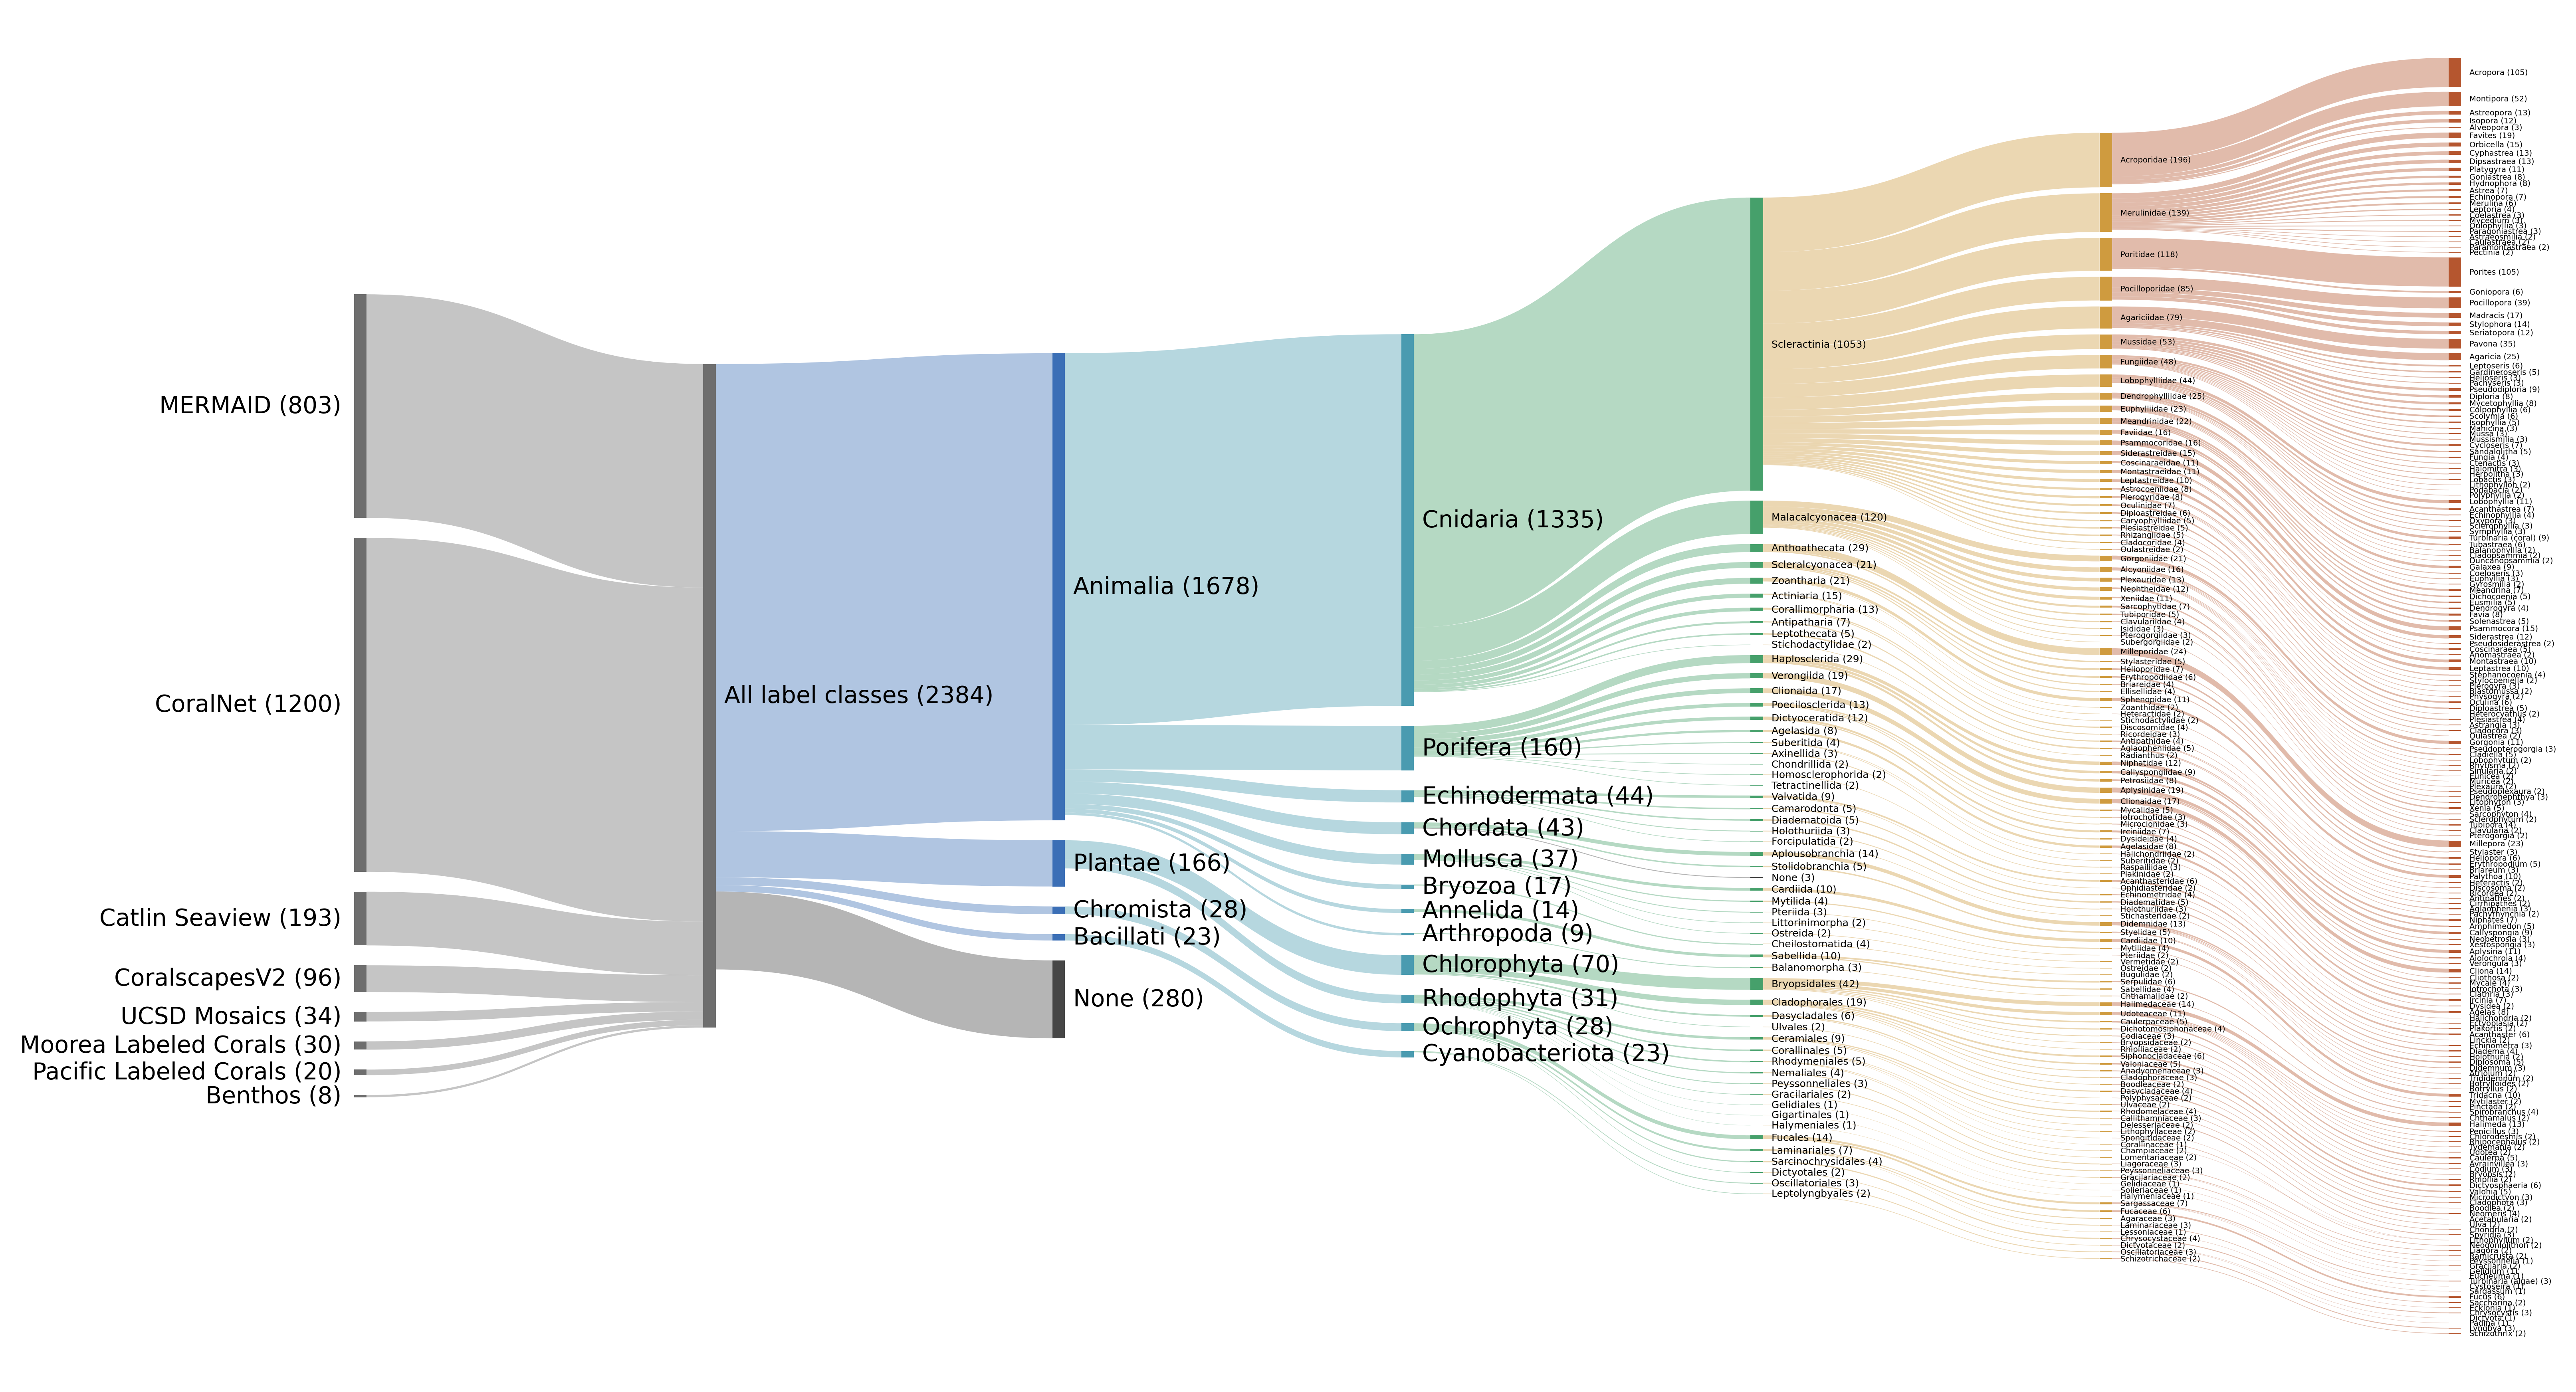
\includegraphics[width=0.99\linewidth]{taxonomy_sankey.png}
    \captionof{figure}{Taxonomic concepts of the mapped label classes. Some label classes explicitly map to ``None'' as the taxonomy, e.g. (``Rock'', or ``Transect tape''). Multiple label classes can map to the same taxonomic concepts (e.g. ``Porites alive'' and ``Porites bleached''). }
    \label{appendix:sankey}
\end{center}
TODO
}]

\twocolumn[{%
\begin{center}
    \pierow{images}\\[2pt]
    \pierow{annotations}\\[2pt]
    \pierow{pixels}\\[4pt]
    \includegraphics{\appfig/legend_datasets.pdf}
    \captionof{figure}{Share of each source dataset in the reconciled data at the source label level (pre-mapping, Tab.~\ref{tab:dataset}). Rows show images, annotations, and annotated pixels; columns show all splits combined and the train, validation, and test splits.}
    \label{fig:appendix_pies}
    \vspace{8pt}
    \includegraphics[width=0.33\textwidth]{\appfig/labels_images.pdf}\hfill
    \includegraphics[width=0.33\textwidth]{\appfig/labels_annotations.pdf}\hfill
    \includegraphics[width=0.33\textwidth]{\appfig/labels_pixels.pdf}
    \captionof{figure}{Heavy-tailed distribution of the source labels that are mapped in our label space, over train, validation, and test combined. Each bar is one source label of one dataset, sorted by the number of images containing it (left), its number of annotations (middle), and its number of annotated pixels (right), and colored by dataset as in Fig.~\ref{fig:appendix_pies}. Note the logarithmic y-axis.}
    \label{fig:appendix_label_hist}
\end{center}
}]

\twocolumn[{%
\begin{center}
    \includegraphics[width=\linewidth]{\appfig/concepts_balance.pdf}
    \captionof{figure}{Share of mapped annotations and annotated pixels for which each health, morphology, and auxiliary concept is true, false, or not given, over train, validation, and test combined. (a) All annotations. (b) All annotated pixels. (c) Cnidarian annotations and (d) Cnidarian annotated pixels use only labels whose phylum is Cnidaria. One annotation is one sparse point or one 8-connected component of a dense mask. Dashed lines separate health, morphology, and auxiliary concepts.}
    \label{fig:appendix_concept_balance}
\end{center}
}]

\twocolumn[{%
\subsection{CoralscapesV2}
TODO: CoralscapesV2 \cite{coralscapesv2} is comprised of TODO images, annotated with TODO polygons, etc...

TODO: histogram of number of labels in dataset
\begin{center}
    \setlength{\appW}{0.19\textwidth}\setlength{\appH}{0.095\textwidth}
    \densegrid{coralscapes_v2}\\[4pt]
    \includegraphics{\appfig/coralscapes_v2/legend_coralscapes_v2.pdf}
    \captionof{figure}{Ten random CoralscapesV2 images, each shown above its dense source-level labels, using the color scheme of \citet{coralscapesv2}. Unlabeled pixels are white.}
    \label{fig:appendix_coralscapes_v2}
\end{center}
}]

\twocolumn[{%
\subsection{CoralNet}
TODO: CoralNet Descriptio
\begin{center}
    \setlength{\appW}{0.125\textwidth}\setlength{\appH}{0.7\appW}
    %\coralnetsource{2236}\\[6pt]
    \coralnetsource{3172}\\[6pt]
    \coralnetsource{3368}\\[6pt]
    \coralnetsource{4495}\\[6pt]
    \coralnetsource{5603}
    \captionof{figure}{Ten random images from random CoralNet sources (labeled with their CoralNet source ID), with the point annotations drawn at the source label level. Each legend lists the labels present in the ten images of its source; labels shared across sources share a color.}
    \label{fig:appendix_coralnet}
\end{center}
}]

\twocolumn[{%
\begin{center}
    \setlength{\appW}{0.125\textwidth}\setlength{\appH}{0.7\appW}
    \coralnetsource{6179}\\[6pt]
    \coralnetsource{6543}\\[6pt]
    \coralnetsource{6695}\\[6pt]
    \coralnetsource{6956}\\[6pt]
    \coralnetsource{7037}
    % Same figure number as the previous page. A real float (and \ContinuedFloat)
    % cannot sit in this box, so step the counter back and give hyperref its own anchor.
    \begingroup
    \addtocounter{figure}{-1}%
    \renewcommand{\theHfigure}{coralnet-continued}%
    \captionof{figure}{CoralNet sources (continued).}
    \endgroup
\end{center}
}]

\twocolumn[{%
\subsection{UCSD Mosaics}
\citep{edwards}

TODO explain the dataset is shit (nicely) and that its available as a pdf where the labels don't match, and that instead we use the version from Reine et al, which discards some corrupted labels.
\begin{center}
    \setlength{\appW}{0.19\textwidth}\setlength{\appH}{\appW}
    \densegrid{ucsd_mosaics}\\[4pt]
    \includegraphics{\appfig/ucsd_mosaics/legend_ucsd_mosaics.pdf}
    \captionof{figure}{Ten random UCSD Mosaics tiles, each shown above its dense source-level labels. Unlabeled pixels are white.}
    \label{fig:appendix_ucsd_mosaics}
\end{center}
}]

\twocolumn[{%
\subsection{Catlin Seaview}
\begin{center}
    \setlength{\appW}{0.19\textwidth}\setlength{\appH}{\appW}
    \sparsegrid{catlin_seaview}\\[4pt]
    \includegraphics{\appfig/catlin_seaview/legend_catlin_seaview.pdf}
    \captionof{figure}{Ten random Catlin Seaview images with their point annotations drawn at the source label level.}
    \label{fig:appendix_catlin_seaview}
\end{center}
}]

\twocolumn[{%
\subsection{Moorea Labeled Corals}
\begin{center}
    \setlength{\appW}{0.19\textwidth}\setlength{\appH}{\appW}
    \sparsegrid{moorea_labeled_corals}\\[4pt]
    \includegraphics{\appfig/moorea_labeled_corals/legend_moorea_labeled_corals.pdf}
    \captionof{figure}{Ten random Moorea Labeled Corals images with their point annotations drawn at the source label level.}
    \label{fig:appendix_moorea}
\end{center}
}]

\twocolumn[{%
\subsection{Pacific Labeled Corals}
TODO: explain how, technically, moorea is technically part of this dataset, but we treat that separately, and don't re-include the moorea split
\begin{center}
    \setlength{\appW}{0.19\textwidth}\setlength{\appH}{0.1425\textwidth}
    \sparsegrid{pacific_labeled_corals}\\[4pt]
    \includegraphics{\appfig/pacific_labeled_corals/legend_pacific_labeled_corals.pdf}
    \captionof{figure}{Ten random Pacific Labeled Corals images with their point annotations drawn at the source label level.}
    \label{fig:appendix_pacific}
\end{center}
}]

\twocolumn[{%
\subsection{MERMAID}
TODO...
\begin{center}
    \setlength{\appW}{0.19\textwidth}\setlength{\appH}{\appW}
    \sparsegrid{mermaid}\\[4pt]
    \includegraphics{\appfig/mermaid/legend_mermaid.pdf}
    \captionof{figure}{Ten random MERMAID images with their point annotations drawn at the source label level.}
    \label{fig:appendix_mermaid}
\end{center}
}]

\twocolumn[{%
\subsection{Benthos}
TODO...

- Drop Orthomosaic from Mediterannean
\begin{center}
    \setlength{\appW}{0.19\textwidth}\setlength{\appH}{\appW}
    \densegrid{benthos_yuval}\\[4pt]
    \includegraphics{\appfig/benthos_yuval/legend_benthos_yuval.pdf}
    \captionof{figure}{Ten random Benthos tiles, each shown above its dense source-level labels. Unlabeled pixels are white.}
    \label{fig:appendix_benthos}
\end{center}
}]

\end{document}
